\section{Using STOQS}

\subsection{Operation}

STOQS has been in use at MBARI for over 3 years to help manage and visualize data collected during upper water column measurement campaigns where scientific goals center on improving our understanding of biological processes. The data consist primarily of measurements collected by moving platforms. The platforms have accurate clocks, Global Positioning Sensors and underwater inertial navigation sensors, and one or more instruments that measure parameters such as temperature, salinity, oxygen, nitrate, chlorophyll fluorescence, optical backscatter, and particle sizes. Some platforms can also capture water samples for later laboratory analysis. A typical workflow for is:
\begin{enumerate}
\item Install the STOQS software on a Linux server
\item Vehicles conduct their missions, collecting data
\item Create NetCDF files of the instrument data
\item Construct and execute a STOQS load script
\item Access and visualize data using the STOQS UI
\end{enumerate}


\subsection{Loading Data}

In the fall of 2013, STOQS was used in the MBARI project CANON: Controlled Agile, and Novel Observing Network, with the goal of 1) using STOQS during an ongoing campaign to assist in making optimal sampling decisions and 2) to train users how to load data.  The CANON project was perfect for this task as there were multiple platforms, multiple institutions, and the need for continual visual analysis during the campaign.  Over 3.4 million data points were loaded from 23 platforms, covering 126 measurements, over a 39 day period. 

The CANON project took place between September 9 to October 16 2014, in and around the Monterey Bay, CA with the following objectives: 
\begin{enumerate}
\item Can we identify and trace source water and seed populations for phytoplankton blooms in and out of Monterey Bay?
\item Can we develop environmental indices that can be used to predict the location and timing of blooms with enough accuracy and speed to be used to trigger autonomous sampling?
\item Can we develop an information processing and display system that can be used in real time to improve decision making and publication preparation in delayed mode?
\end{enumerate}

To this end, a total of 27 platforms participated in the campaign: 4 ships, 3 AUVs, 8 gliders, 7 drifters, and 5 moorings.  Fig.~\ref{fig:ReikoFigure1} shows the location and tracks of the platforms.

\begin{figure}[htbp]
\centering
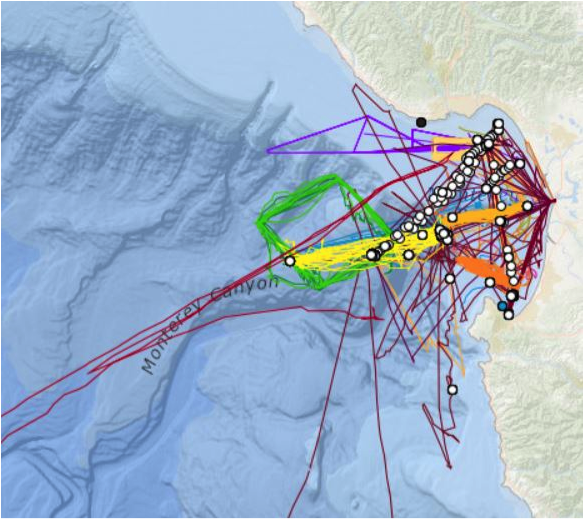
\includegraphics[width=3.3in]{ReikoFigure1.png}
\caption{STOQS map of the platforms used in the CANON Fall 2013 campaign in Monterey Bay, Central California.}
\label{fig:ReikoFigure1}
\end{figure}

Data from the platforms were received through a variety of portals and the data were in varying states of processing.  Some data were received hourly and other data on a daily basis.  The goal was to process the data as soon as possible and load it into STOQS for decision making analysis.  The process was automated for all platforms, except for the ships, using cron scripts.  For STOQS loading, all data is required to be in NetCDF format.  Compliance with CF naming standards is needed to allow interaction between parameters from different platforms.  After raw data processing and NetCDF conversion, all data was loaded onto the CANON data repository, a THREDDS Server.  A Test STOQS installation was set up for the trainees where new load functions could be tested before loading to the production STOQS installation.   Fig.~\ref{fig:ReikoFigure2} illustrates the data flow.

\begin{figure}[htbp]
\centering
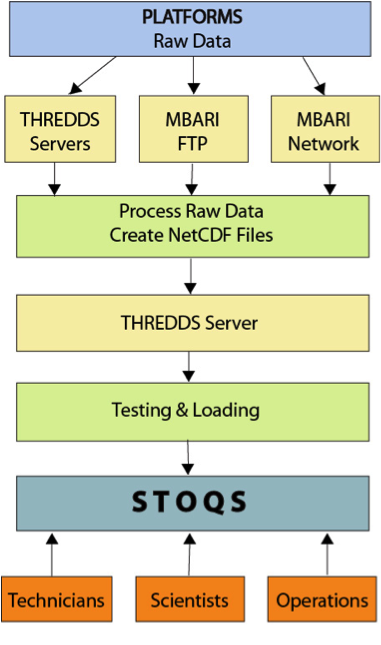
\includegraphics[width=2.5in]{ReikoFigure2.png}
\caption{Data flow.}
\label{fig:ReikoFigure2}
\end{figure}

STOQS is an open source project available on https://code.google.com/p/stoqs/.  Detailed load instructions can be found at https://code.google.com/p/stoqs/source/browse/LOADING.  In the MBARI CANON STOQS installation the following directory structure was setup (Fig.~\ref{fig:ReikoFigure3}).  Project loading scripts and individual platform loading scripts are under the loaders/ subdirectory,  CANON/ The subdirectory toNetCDF/ contain the python programs to convert data to NetCDF.  

\begin{figure*}[htbp]
\centering
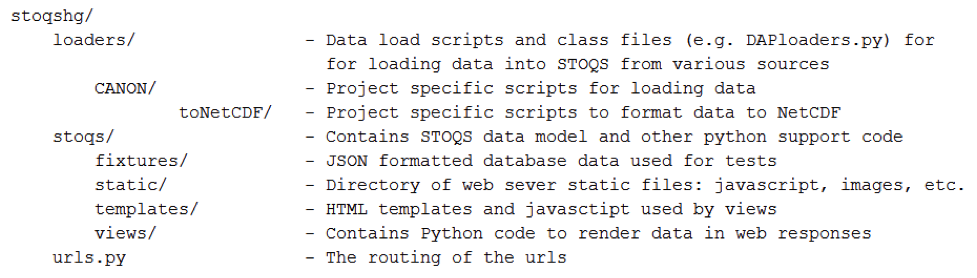
\includegraphics[width=5.0in]{ReikoFigure3.png}
\caption{STOQS installation directory structure. The subdirectories CANON/ and toNetCDF/ contain project specific  scripts for loading and converting data.}
\label{fig:ReikoFigure3}
\end{figure*}

Samples of python loading scripts can be found in the loaders/ project specific subdirectories, such as loaders/CANON/. Similarly python conversion scripts can be found under the toNetCDF/ subdirectories.  The following section briefly describes the loading steps and includes relevant sections of code. 

\begin{figure}[htbp]
\centering
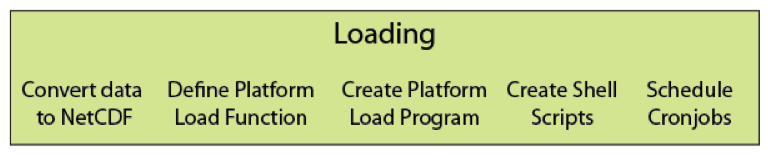
\includegraphics[width=3.3in]{ReikoFigure4.png}
\caption{Loading steps.}
\label{fig:ReikoFigure4}
\end{figure}

To load a platform there must be the following:

\begin{itemize}
\item NetCDF formatted data
\item Platform load functions
\item Platform load programs
\end{itemize}

Fig.~\ref{fig:ReikoFigure5} is an example of the script used to download profiling CTD data from a ship, convert the data files to NetCDF, and upload the converted files to the project’s data repository.

\begin{figure}[htbp]
\centering
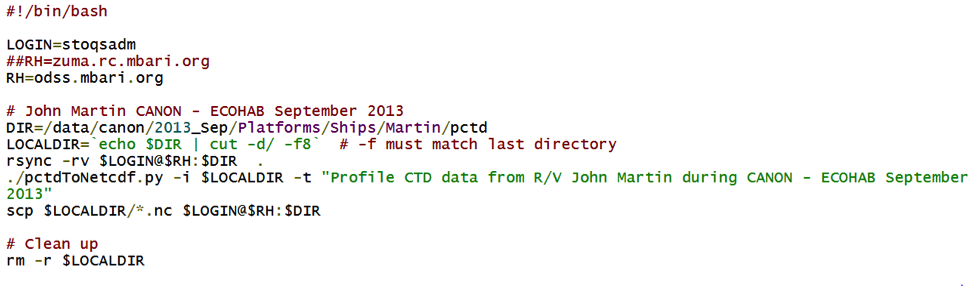
\includegraphics[width=3.3in]{ReikoFigure5.png}
\caption{Shell script used to convert shipboard CTD data to NetCDF.}
\label{fig:ReikoFigure5}
\end{figure}

Platform load functions are defined in the CANONLoader class in the python file /loaders/\_\_init\_\_.py   A load function is created for each distinct platform.  Fig.~\ref{fig:ReikoFigure6} is the load function for the AUV Dorado.  The platform load script will call this function and pass the parameters to begin loading Dorado data.  One may maintain a full and strided database.  A strided data load is subsampled for quick exploration.

\begin{figure}[htbp]
\centering
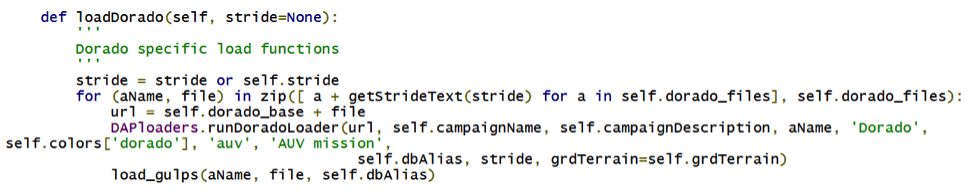
\includegraphics[width=3.3in]{ReikoFigure6.png}
\caption{AUV load function from the CANONLoader class.}
\label{fig:ReikoFigure6}
\end{figure}

The third loading step is creating a python load program.  The location of the data and the data files to load are defined and passed to the function loadDorado.  Fig.~\ref{fig:ReikoFigure7} is the code defining parameters for the AUV Dorado and the command call.

\begin{figure*}[htbp]
\centering
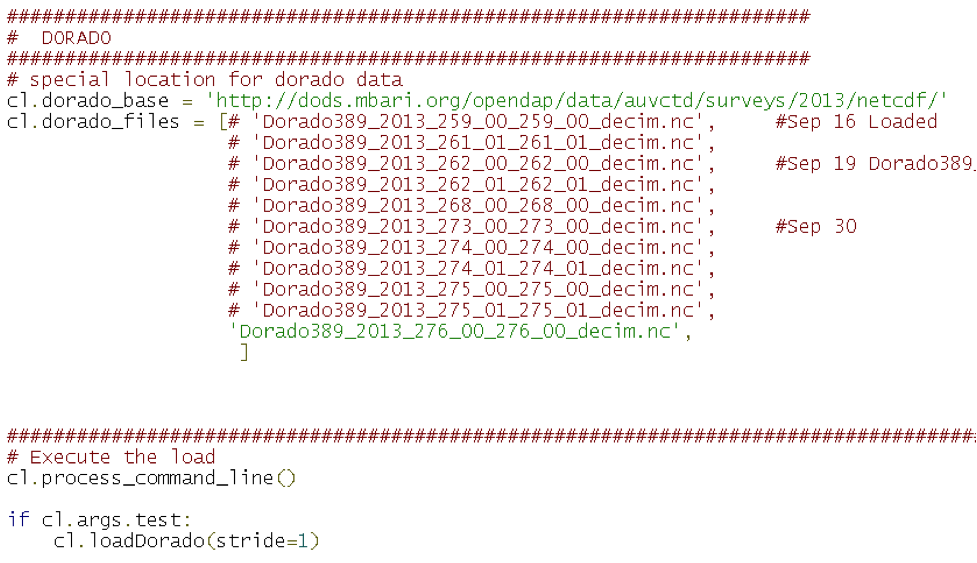
\includegraphics[width=6.6in]{ReikoFigure7.png}
\caption{Python code for AUV data load.}
\label{fig:ReikoFigure7}
\end{figure*}

One of the requirements for using STOQS in the CANON campaign was to assist in decisions as the project was ongoing. Quick exploration and visual analysis helped the team to assess the environmental conditions to guide where to send the AUVs, ships, and gliders.  The CANON project included platforms that were able to sample on a 24 hours basis, LRAUVs, moorings, drifters, and gliders.  Our goal was to load the data as soon as possible. We automated the loading using shell scripts scheduled to run using cron.  Fig.~\ref{fig:ReikoFigure8} is an example of the shell script used to run the glider loading.


\begin{figure}[htbp]
\centering
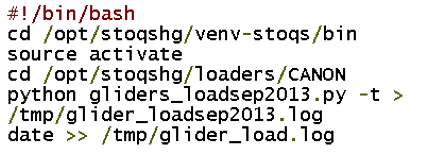
\includegraphics[width=2.3in]{ReikoFigure8.png}
\caption{Glider shell script to run the glider data load.}
\label{fig:ReikoFigure8}
\end{figure}

The crontab in Fig.~\ref{fig:ReikoFigure9} illustrates the loading of the OA mooring, the ESP mooring, and the Stella drifters on a two hour schedule.

\begin{figure*}[htbp]
\centering
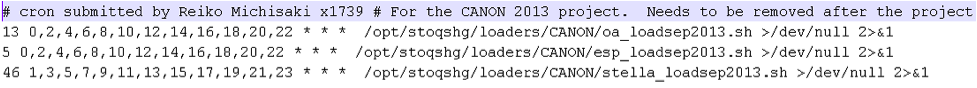
\includegraphics[width=6.6in]{ReikoFigure9.png}
\caption{Crontab schedule to run platforms.}
\label{fig:ReikoFigure9}
\end{figure*}

In addition to individual loading of platforms, post campaign a master loading script was developed to load all the platform data at once.  This allows custom striding of data, the loading of quality controlled data, and a clean loading of all data sets.  In conclusion, the trainees were able to successfully load CANON campaign data.  Science was able to use the analytical tools to study biological dynamics, and engineers were able to monitor platform and sensor performance.  

[a figure of STOQS output, like glider or auv tracks with the spatial map and the timeline graphs]



\subsection{Exploring Data}
Collecting high-resolution sections of multidisciplinary data, AUVs offer great potential for understanding marine ecology.  Yet the density and complexity of AUV data challenge efficient and effective exploration.  STOQS is facilitating exploration of AUV data from a variety of experiments.  Here we present an example exploration of AUV data in phytoplankton ecology research.

Occupying the core of the oceanic food web, phytoplankton (microscopic algae) are essential to ocean life, and their photosynthesis supplies about half of humanity’s oxygen needs.  While essential to earth’s biosphere, a small percentage of phytoplankton species can cause harm, for example by producing substances that are toxic to marine life and people.  Studying the ecology of harmful algal blooms (HABs) requires interdisciplinary research over a range of spatial and temporal scales, and AUVs provide excellent observations of phytoplankton patchiness and its relationship to environmental conditions at small to regional scales.  Some AUVs can also acquire whole water samples autonomously targeted on phytoplankton patches, from which subsequent laboratory analyses can reveal phytoplankton identity and toxicity.  Supporting this research, STOQS integrates AUV data on the environment, optical characteristics of the phytoplankton, locations of sampling, and the data derived from shore-side laboratory analyses.

An experiment conducted during fall 2013 in Monterey Bay, California focused on HAB ecology, and it heavily employed AUVs (Fig.~\ref{fig:ReikoFigure1}).  

One of the primary HAB ecological questions concerns the source of seed populations for bloom events.  Seed populations for blooms may originate within our outside of Monterey Bay.  The first survey by a water-sampling AUV identified spatially separated phytoplankton populations within and outside the bay (Fig.~\ref{fig:JohnsFigureY}, top panel).  The population outside the bay had much higher chlorophyll fluorescence (left).  The separated phytoplankton populations occupied water of significantly different salinity (Fig.~\ref{fig:JohnsFigureY}, bottom panel), indicative of different ecological histories.

\begin{figure}[htbp]
\centering
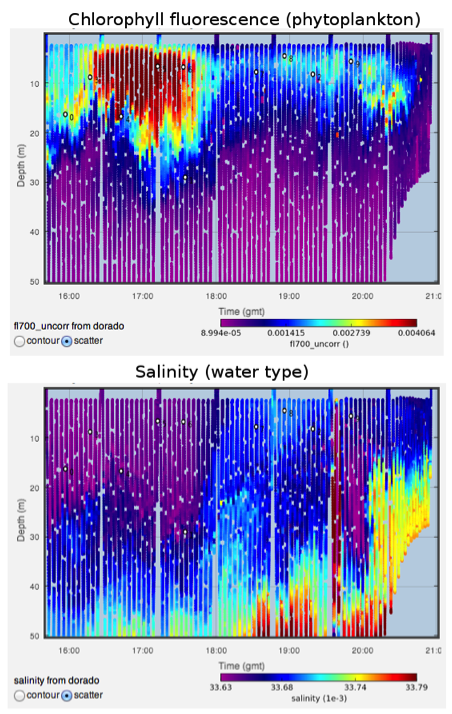
\includegraphics[width=3.3in]{JohnsFigureY.png}
\caption{Vertical sections of chlorophyll fluorescence (top) and salinity (bottom) for an AUV section from offshore (left) to onshore (right) across northern Monterey Bay on 16 September 2013.}
\label{fig:JohnsFigureY}
\end{figure}

Property-property plotting revealed that the spatially separated phytoplankton populations exhibited different optical properties.  The offshore patch exhibited a higher ratio of chlorophyll fluorescence to optical backscattering (Fig.~\ref{fig:JohnsFigureZ}, high-chlorophyll points identified by the lowest salinity values).

Water samples were acquired by the AUV from both phytoplankton populations (white circles in Fig.~\ref{fig:JohnsFigureY}).  Examination of these samples by microscopy revealed elevated abundances of a toxigenic species of diatom in the offshore patch.  This simple exploration thus represents the potential for developing optical proxies for phytoplankton ecotypes, as a tool for not only interpretation of data, but also refinement of autonomously targeted sampling by AUVs using optical data in real-time to control sample acquisition.

\begin{figure}[htbp]
\centering
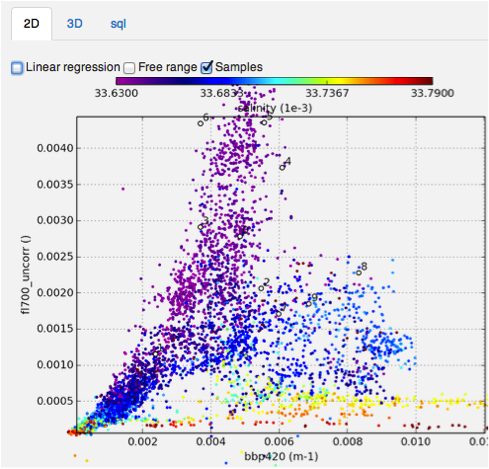
\includegraphics[width=3.3in]{JohnsFigureZ.png}
\caption{STOQS plot of the relationship between optical backscattering (x) and chlorophyll fluorescence (y), colored by salinity, for the AUV section shown in Fig.~\ref{fig:JohnsFigureY}.}
\label{fig:JohnsFigureZ}
\end{figure}

Beyond this simple illustration of AUV data exploration, the fusion of data from many other experiment platforms allows researchers to relate the AUV data to many other observations.

